\chapter{Lua Environment} \label{lua}

Currently, web browser cannot execute lua code, as lua environment is not readily available in browser. So, to handle execution of lua into the browser, javascript implementation of lua interpreter is necessary. 

For this project, to provide lua support for browser, we will use lua VM on the web \cite{luavm}. The VM will create lua environment, where we will be able to execute our program written in lua.

\section{The Lua VM}

The Lua VM runs on the browser, by porting entire ANSI C implementation of lua virtual machine to Java Script using Emscripten \cite{emscripten} including garbage collection.

The Lua VM can be added on to the web page, by referencing lua.vm.js script on the browser, as shown below, 


\begin{lstlisting}[frame=single]  
<html>
  <head>
    <script src="lua.vm.js"></script>
  </head>
</html>
\end{lstlisting}

Once, instance of Lua VM is added on the web page, we can start writtng our lua code in the web page, by including all the lua code into text/lua script as shown below, 

\begin{lstlisting}[frame=single]  
<script type="text/lua">
  ...your lua code
</script>
\end{lstlisting}

Lua VM interpretes the code written in "$<$script type="text/lua" $>$ $<$/script$>$" tags, and it executes it as lua code.

\subsection{Examples}

In this section, we will see some of the examples using lua VM into browser.

\textbf{1. Showing alert on the web page using lua}

Following example renders alert method of javascript global object using lua.  

\begin{lstlisting}[frame=single]
<html>
<head>
<script src="lua.vm.js"></script>

<script type="text/lua">
js.global:alert('hello from Lua script tag in HTML!')
</script>

</head>
<body>
Lua in browser.
</body>
</html>
\end{lstlisting}

\textbf{Output}

Executing above, code into browser generates the output similar to calling alert function from DOM, as shown in figure \ref{fig:luaalert}, 

\begin{figure}[H]
	\begin{center}
		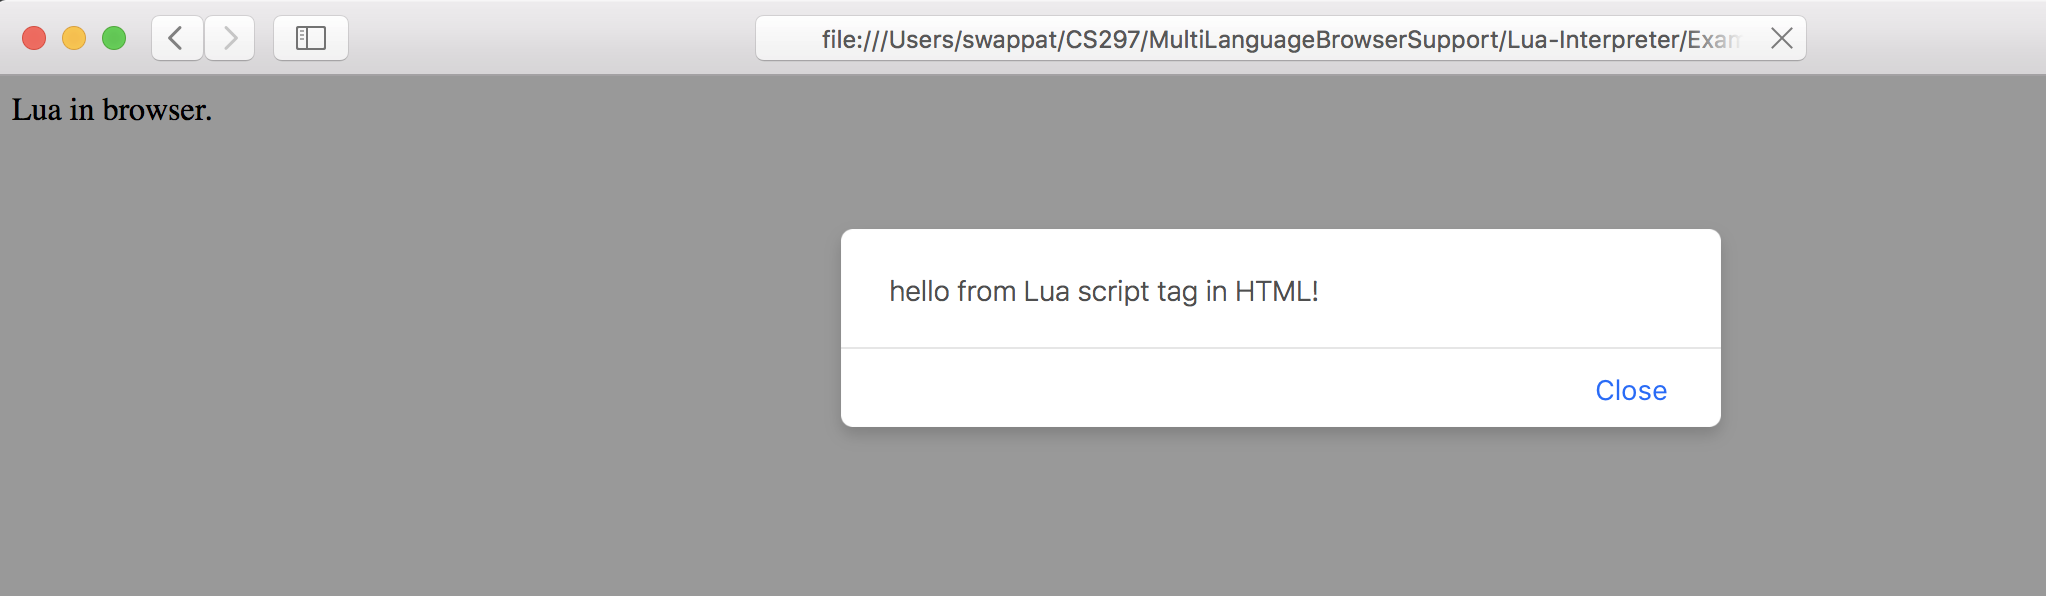
\includegraphics[width=\linewidth]{./images/lua-alert.png}
	\end{center}
	\caption{Showing alert on the web page using lua : Output}
	\label{fig:luaalert}
\end{figure}

\textbf{2. Executing lua function into browser}

We can also define and call lua function in the web page, as shown below,

\begin{lstlisting}[frame=single]  
<html>
<head>
<script src="lua.vm.js"></script>
<title>Lua VM </title>
<script type="text/lua">
  -- function
  function printName (recipient)
    print('Hello, '..recipient)
  end
  -- Anonymus function
  local sayHello = function (recipient)
    print('Hello, '..recipient)
  end
  sayHello('Swapnil')
  printName('CS298 Project')
</script>
</head>
<body>
  Executing lua function in browser.
</body>
</html>
\end{lstlisting}

\textbf{Output}

Executing above code in the browser, creates function called "printName" and assigns anonymous function to local variable "sayHello". After calling the both the functions, we see the desired output on the console, as shown in figure \ref{fig:luafunction}

\begin{figure}[H]
	\begin{center}
		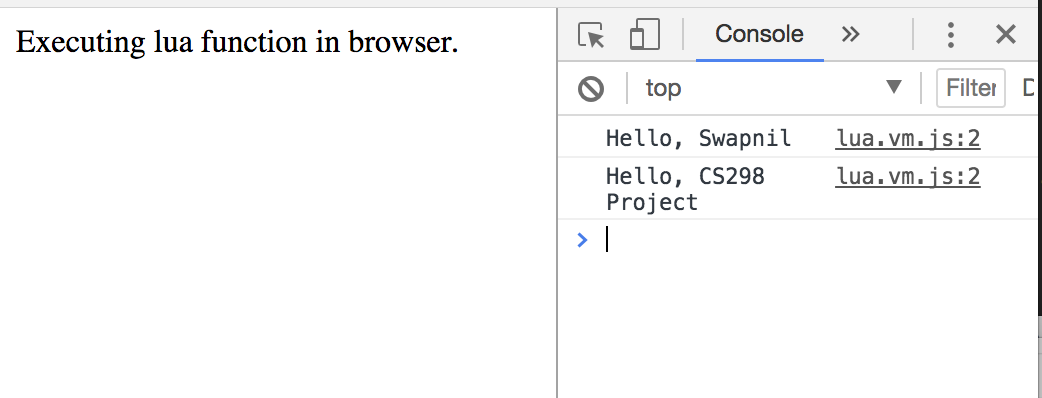
\includegraphics[width=\linewidth]{./images/lua-functions.png}
	\end{center}
	\caption{Executing lua function into browser : Output}
	\label{fig:luafunction}
\end{figure}


\section{Approches}

Similar to scheme environment, we implemented two ways to include lua.vm into the web page, to help browser undderstand lua code on the page.


\subsection{Browser Plugin } 
For this approach, browser plugin (supported by firefox, and chrome) will push the instance of lua VM into every newly opened browser tab. In this way, user don't have to worry about adding the library script on the page. Lua VM library will then interpret all the code enclosed within "type=text/lua" script.

In case of using browser plugin,our example code to render alert on browser will look like, 

\begin{lstlisting}[frame=single]
<html>
<head>
<script type="text/lua">
js.global:alert('hello from Lua script tag in HTML!') 
</script>
</head>
<body>
Lua in browser.
</body>
</html>
\end{lstlisting}


As shown in the code snippet above, we don't need to add any external libraries into our webpage, to interpret lua script. Browser plugin will take care of that.
Executing above code in browser with our plugin installed, will alert user with "hello from Lua script tag in HTML!'" as text.


\subsection{JS Library}


In this approach, lua VM support is achieved in web pages by including lua VM library in web page itself. When web page will loaded into browser,  library will read code snippet inside "type=text/lua" script and will interpret it, as shown in the "Showing alert on the web page using lua" example in examples section. 
